%%%%%%%%%%%%%%%%%%%%%%%%%%%%%%%%%%%%%%%%%%%%%%%%%%%%%%%%%%%%%%%
%
% Welcome to Overleaf --- just edit your LaTeX on the left,
% and we'll compile it for you on the right. If you give 
% someone the link to this page, they can edit at the same
% time. See the help menu above for more info. Enjoy!
%
%%%%%%%%%%%%%%%%%%%%%%%%%%%%%%%%%%%%%%%%%%%%%%%%%%%%%%%%%%%%%%%

%  My thanks to Dana Ernst of Northern Arizona University for sharing 
%    his template with me. This is largely his work.
% --------------------------------------------------------------
% This is all preamble stuff that you don't have to worry about.
% Head down to where it says "Start here"
% --------------------------------------------------------------
 
\documentclass[12pt]{article}
 
\usepackage[margin=1in]{geometry} 
\usepackage{amsmath,amsthm,amssymb}
\usepackage{graphicx}
\usepackage{float}
\usepackage[table,x11names]{xcolor}
\usepackage[lined, linesnumbered]{algorithm2e}
\usepackage{tikz}
\makeatletter
\newenvironment{btHighlight}[1][]
{\begingroup\tikzset{bt@Highlight@par/.style={#1}}\begin{lrbox}{\@tempboxa}}
{\end{lrbox}\bt@HL@box[bt@Highlight@par]{\@tempboxa}\endgroup}

\newcommand\btHL[1][]{%
  \begin{btHighlight}[#1]\bgroup\aftergroup\bt@HL@endenv%
}
\def\bt@HL@endenv{%
  \end{btHighlight}%   
  \egroup
}
\newcommand{\bt@HL@box}[2][]{%
  \tikz[#1]{%
    \pgfpathrectangle{\pgfpoint{1pt}{0pt}}{\pgfpoint{\wd #2}{\ht #2}}%
    \pgfusepath{use as bounding box}%
    \node[anchor=base west, fill=orange!30,outer sep=0pt,inner xsep=1pt, inner ysep=0pt, rounded corners=3pt, minimum height=\ht\strutbox+1pt,#1]{\raisebox{1pt}{\strut}\strut\usebox{#2}};
  }%
}
\makeatother

\usepackage[listings,skins]{tcolorbox}
\tcbset{colback=gray!1!white,colframe=black}




\newenvironment{theorem}[2][Theorem]{\begin{trivlist}
\item[\hskip \labelsep {\bfseries #1}\hskip \labelsep {\bfseries #2.}]}{\end{trivlist}}
\newenvironment{lemma}[2][Lemma]{\begin{trivlist}
\item[\hskip \labelsep {\bfseries #1}\hskip \labelsep {\bfseries #2.}]}{\end{trivlist}}
\newenvironment{conjecture}[2][Conjecture]{\begin{trivlist}
\item[\hskip \labelsep {\bfseries #1}\hskip \labelsep {\bfseries #2.}]}{\end{trivlist}}
\newenvironment{question}[2][Question]{\begin{trivlist}
\item[\hskip \labelsep {\bfseries #1}\hskip \labelsep {\bfseries #2.}]}{\end{trivlist}}
\newenvironment{corollary}[2][Corollary]{\begin{trivlist}
\item[\hskip \labelsep {\bfseries #1}\hskip \labelsep {\bfseries #2.}]}{\end{trivlist}}
\newenvironment{definition}[2][Definition]{\begin{trivlist}
\item[\hskip \labelsep {\bfseries #1}\hskip \labelsep {\bfseries #2.}]}{\end{trivlist}}


\definecolor{commentgreen}{RGB}{176, 176, 176}
\definecolor{rowcolor}{cmyk}{0,0.87,0.68,0.32}
\definecolor{rowcolor2}{cmyk}{ 20, 0, 37, 34}

\definecolor{eminence}{RGB}{108,48,130}
\definecolor{weborange}{RGB}{255,165,0}
\definecolor{frenchplum}{RGB}{129,20,82}
\definecolor{darkgreen}{RGB}{10, 92, 10}


\definecolor{celadon}{rgb}{0.67, 0.88, 0.69}

\definecolor{mGreen}{rgb}{0,0.6,0}
\definecolor{mGray}{rgb}{0.5,0.5,0.5}
\definecolor{mPurple}{rgb}{0.58,0,0.82}
\definecolor{backgroundColour}{rgb}{0.95,0.95,0.92}

\lstdefinestyle{CStyle}{
    commentstyle=\color{mGreen},
    keywordstyle=\color{magenta},
    numberstyle=\tiny\color{mGray},
    stringstyle=\color{mPurple},
    basicstyle=\footnotesize,
    breakatwhitespace=false,         
    breaklines=true,                 
    captionpos=b,                    
    keepspaces=true,                 
    numbers=left,                    
    numbersep=5pt,                  
    showspaces=false,                
    showstringspaces=false,
    showtabs=false,                  
    tabsize=2,
    language=C,
    moredelim=**[is][{\btHL[celadon!40]}]{`}{`}
}

\lstdefinestyle{nccode}{
    numbers=none,
    stepnumber=1,
    numbersep=10pt,
    tabsize=4,
    showspaces=false,
    breaklines=true, 
    showstringspaces=false,
    moredelim=**[is][{\btHL[orange!50]}]{`}{`}
}

\begin{document}
 
% --------------------------------------------------------------
%                         Start here
% --------------------------------------------------------------
 
\title{Assignment 2: Programming with OpenMP} % replace with an appropriate title, choose something shortish & descriptive
\author{Javier Cabrera Arteaga, Deepika Tiwari} % replace with your name, multiple authors go in alphabetical order by last name
 
\maketitle

{%
\centering
FDD3258 - Introduction to High-Performance Computing
\par
}
\hrule
\vspace{.2in}


\section{Exercise 1 - OpenMP Hello World, get familiar with OpenMP Environment}


\begin{enumerate}
	\item Write an OpenMP C code with each thread printing Hello World from Thread X! where X is the thread ID.\\
	\begin{lstlisting}[style=CStyle]
#include <omp.h>
#include <stdio.h>

int th_id, nthreads;

int main(void){

	#ifdef NUM_THREADS
		omp_set_num_threads(NUM_THREADS);
	#endif

	#pragma omp parallel private(th_id)
	{
		nthreads = omp_get_num_threads();
		th_id = omp_get_thread_num();
		printf("Hello, world %d/%d. \n", th_id, nthreads);
	}

	return 0;
}
	\end{lstlisting}
	\item Answers
	\begin{enumerate}
	   \item Compiling:
	       \begin{enumerate}
	           \item To enable openmp in our local machine (MacBook), we compile the above program with \texttt{gcc-9 -fopenmp hello.c -o hello.out}.
		        \item To enable openmp on Beskow, we compile the above program with \texttt{cc -fopenmp hello.c -o hello.out}
	       \end{enumerate}
	    \item Running the program on Beskow
	    \begin{enumerate}
	        \item Request for allocation: \texttt{salloc --nodes=1 -t 00:05:00 -A edu20.fdd3258}
	        \item Run: \texttt{srun -n 1 ./hello.out}
	    \end{enumerate}
	    \item Setting the number of threads:
		    \begin{enumerate}
    			\item Before compiling, set the environment variable with\\
    			\texttt{export OMP\_NUM\_THREADS=<num\_threads>}
    			\item At runtime \texttt{omp\_set\_num\_threads()}
		\end{enumerate}
	\end{enumerate}
	
  
\end{enumerate}

\section{Exercise 2. STREAM benchmark and the importance of threads}
We run the given STREAM benchmark program, for which the schedule was set as guided \texttt{(\#pragma omp parallel for schedule(guided))} five times on Beskow. The mean bandwidth for the copy kernel across a default value of 64 threads, and across the five runs was 48714.62 MB/s and the standard deviation was 137.66.
	\begin{enumerate}
		\item \textit{Prepare a plot (with Excel, Matlab, Gnuplot, …) comparing the bandwidth using 1-2-4-8-12-16-20-24-28-32 threads.}
		
		\begin{figure}[H]
			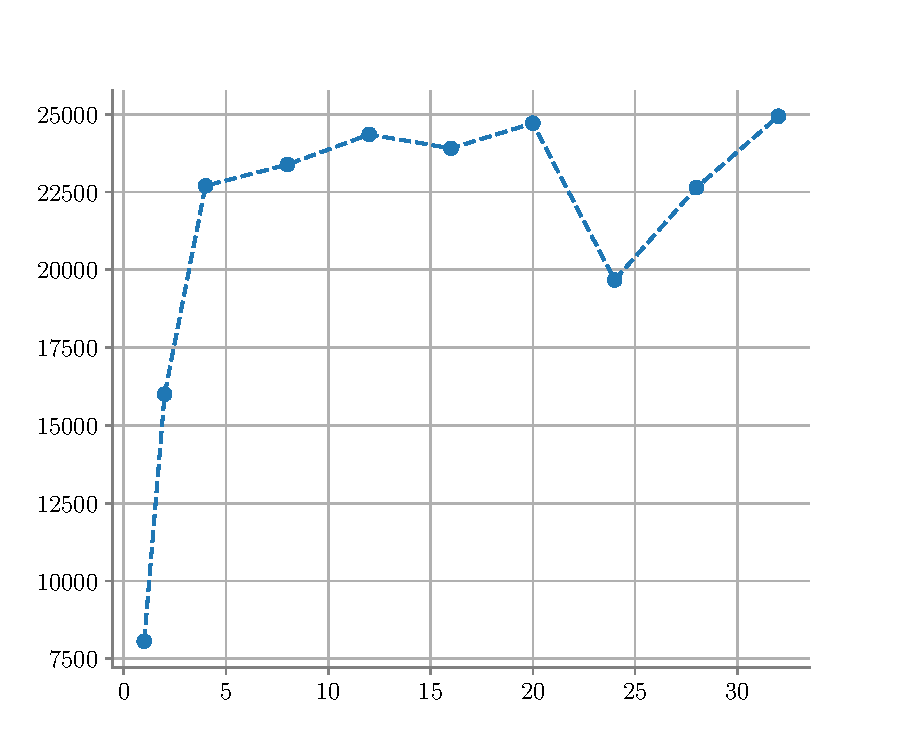
\includegraphics[width=0.8\textwidth]{stream.pdf}
		\end{figure}
		\item \textit{How does the bandwidth measured with copy kernel depend on the number of threads?}
		The bandwidth of the copy kernel in STREAM increases as we increase the number of threads up to a certain threshold, and then flattens out. Adding more threads after an optimal number of threads increases overhead as all the threads have to access the same shared memory system, which itself has a finite bandwidth.
		\item \textit{Prepare a plot comparing the bandwidth measured with copy kernel with static, dynamic and guided schedules using 32 threads.}
		\begin{figure}[H]
			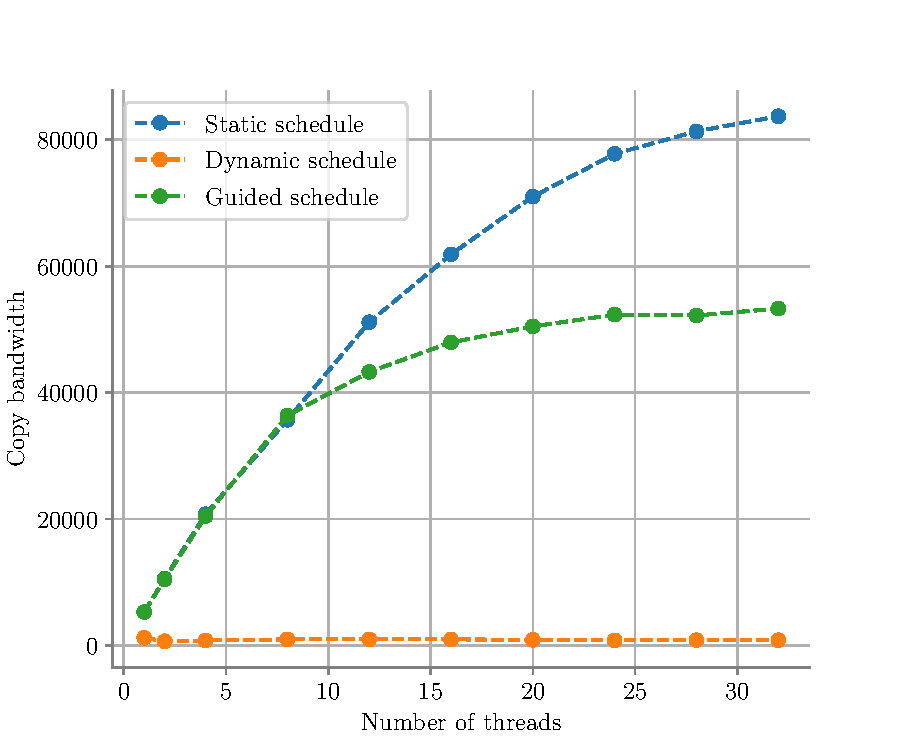
\includegraphics[width=0.8\textwidth]{stream2.pdf}
		\end{figure}
		\begin{enumerate}
			\item \textit{How do you set the schedule in the STREAM code? What is the fastest schedule and why do you think it is so?}\\
			The schedule can be changed by stating the kind of schedule with \texttt{\#pragma omp parallel for schedule(kind(,chunksize))} (line 314 in stream.c).\\
			For the copy kernel in STREAM, the kind of schedule that offers the highest bandwidth is static. This is because the computation performed by each thread is the same - that is copying a part of the source array into the destination array - which is an ideal situation to use static scheduling. Static scheduling adds the least overhead and is a good fit for cases where the thread workloads are mostly balanced.
		\end{enumerate}
	\end{enumerate}

\section{Exercise 3. Maxloc, parallel for, race condition atomic, critical and false sharing}
\begin{enumerate}
    \item \textit{Measure the performance of the serial code (average + standard deviation)}\\
    The average performance of the serial code across five runs on Beskow was found to be 0.0084714s and the standard deviation was 0.000562.\\
    
    \begin{lstlisting}[style=CStyle]
int max() {
	for (int i=0; i < N; i++){
		if (x[i] > maxval)  {
			maxval = x[i]; maxloc = i;
		}
	}
}

\end{lstlisting}
    \item \textit{Use omp parallel for construct to parallelize. Run the code with 32 threads and measure the execution time (average + standard deviation). Is the code correct? If not, why so?}\\
    The average performance with the \texttt{\#pragma omp parallel for} construct is 0.0026814s and the standard deviation was 0.000049\\
    The problem with this code is that multiple threads potentially write to the shared variable maxval and maxloc at the same time.\\
    
    \begin{lstlisting}[style=CStyle]
int maxOmpNoCriticalSection() {
	omp_set_num_threads(NTHREADS);
	#pragma omp parallel for
	for (int i=0; i < N; i++){
		if (x[i] > maxval) {
			maxval = x[i]; maxloc = i;
		}
	}
}
    \end{lstlisting}
    \item \textit{Use omp critical  to protect the code region that might be updated by multiple threads concurrently. Measure the execution time for both versions (omp critical) varying the number of threads: 1,2,4,8,16, 20, 24, 28 and 32. How does the performance compare to 1 and 2? What is the reason for the performance gain/loss?}\\
    We add a critical section construct to ensure that only thread can modify variables maxloc and maxval at one time. We vary the number of threads from 1 to 32 as specified. In all cases, we observe that adding a critical section decreases performance (slower execution times) as compared to cases 1 and 2. This is because threads must now wait for another thread to exit the critical section before they can enter it.\\
    
    \begin{lstlisting}[style=CStyle]
int maxOmpCriticalSection(){
	omp_set_num_threads(NTHREADS);
	#pragma omp parallel for
	for (int i=0; i < N; i++){
		#pragma omp critical 
		{
			if (x[i] > maxval) {
				maxval = x[i]; maxloc = i;
			}
		}
	}
}
    \end{lstlisting}
    \item \textit{Try to avoid the use of critical section. Let each thread find the maxloc in its own data then combine their local result to get the final result. For instance, we can use temporary arrays indexed by thread number to hold the values found by each thread. Measure the performance of the new implementation varying the number of threads: 1,2,4,8,16, 20, 24, 28 and 32. Does the performance increase as expected? If not why?}\\
    An alternative to using critical sections is to allow threads to find maxloc and maxval for the section of the array they are working on and saving these results in temporary arrays. These temporary arrays have values corresponding to one thread each and can then be serially accessed to find the actual values for maxval and maxloc. This strategy eliminates the need for maintaining a critical section, thus reducing the corresponding overhead and leading to an overall increase in performance.\\
    
    \begin{lstlisting}[style=CStyle]
double maxValues[NTHREADS];
int maxLocs[NTHREADS];
int maxOmpTempIndexes(){
	omp_set_num_threads(NTHREADS);
	int th_id;
	#pragma omp parallel for private(th_id)
	for (int i=0; i < N; i++){
		th_id = omp_get_thread_num();
		
		if (x[i] > maxValues[th_id]) {
			maxValues[th_id] = x[i]; maxLocs[th_id] = i;
		}
	}
	for(int i = 0; i < NTHREADS; i++)
		if (maxValues[i] > maxval) {
				maxval = maxValues[i]; maxloc = maxLocs[i];
		}
}
    \end{lstlisting}
    \item \textit{Write a version of the code in 4 using a technique to remove false sharing with padding. Measure the performance of code varying the number of threads: 1,2,4,8,16, 20, 24, 28 and 32.}\\
    False sharing can be caused when two threads access and modfiy different variables that happen to lie on the same cache line. The result is that whenever one thread modifies the variable it has access to, the cache line is revalidated, implying that the other variable must also be revalidated even though it may not have been changed. One solution to eliminate false sharing is by the use of some amount of padding so that two variables (arrays, in our example) do not share the same cache line. For the specified number of threads, we observe that the performance improves slightly as compared to case 4. \\
    \begin{lstlisting}[style=CStyle]
#define PAD 512
typedef struct {
	double val;
	int loc;
	char padding[PAD];
} MAXINFO;
MAXINFO infos[NTHREADS];
int maxOmpTempIndexesPadding() {
	omp_set_num_threads(NTHREADS);
	int th_id;

	#pragma omp parallel for private(th_id)
	for (int i=0; i < N; i++){
		th_id = omp_get_thread_num();
		if (x[i] > infos[th_id].val) {
			infos[th_id].val = x[i]; infos[th_id].loc = i;
		}
	}
	for(int i = 0; i < NTHREADS; i++)
		if (infos[i].val > maxval) {
				maxval = infos[i].val; maxloc =infos[i].loc;
		}
}
    \end{lstlisting}
\end{enumerate}
\section{Exercise 4. DFTW, The Fastest DFT in the West}
\begin{enumerate}
    \item \textit{Parallelize the DFTW code with OpenMP. You can develop different strategies; the important point is that the code produces the correct results and it is fast!}\\
    To parallelize the DFT implementation, we maintain a temporary array of structures for each thread that holds the computed real and imaginary values, and some padding to ensure there is no unnecessary cache revalidation. For each value of N (the input size), we first initialize with zero the temporary arrays to store the real and imaginary values of the output vector. Next, we divide the workload (computation of the real and imaginary vectors) equally among a certain number of threads. These values get stored in the temporary arrays of each thread. Finally, we aggregate the values in the temporary arrays by adding them to obtain the final output vectors.\\
    \begin{lstlisting}[style=CStyle]
typedef struct {
  double r;
  int i;
  char padding[PAD];
} TMPINFO;
// DFT/IDFT routine
// idft: 1 direct DFT, -1 inverse IDFT (Inverse DFT)
int DFT(int idft, double* xr, double* xi, double* Xr_o, double* Xi_o, int N){
  omp_set_num_threads(NTHREADS);
  TMPINFO* tmp = (TMPINFO *) malloc(NTHREADS*sizeof(TMPINFO));
  for (int k=0 ; k<N ; k++) {
    for(int i = 0; i < NTHREADS; i++) {
      tmp[i].r = 0.0;
      tmp[i].i = 0.0;	
    }
  
  #pragma omp parallel for schedule(static)
    for (int n=0; n < N  ; n++)  {
      // Real part of X[k]
      int id = omp_get_thread_num();
      tmp[id].r += xr[n] * cos(n * k * PI2 / N) + idft*xi[n]*sin(n * k * PI2 / N);
      // Imaginary part of X[k]
      tmp[id].i += -idft*xr[n] * sin(n * k * PI2 / N) + xi[n] * cos(n * k * PI2 / N);
    }
    for(int i = 0; i < NTHREADS; i++){
      Xr_o[k] += tmp[i].r;
      Xi_o[k] += tmp[i].i;	
    }
  }
  free(tmp);
  // normalize if you are doing IDFT
  if (idft==-1) {
    for (int n=0 ; n<N ; n++){
      Xr_o[n] /=N;
      Xi_o[n] /=N;
    }
  }
  return 1; 
}
    \end{lstlisting}
    
    \item \textit{Measure the performance on Beskow 32 cores reporting the average values and standard deviation for DFTW using an input size equal to 10000 (N=10000).}\\
    The average execution time across 10 runs for prallelized DFTW for 32 threads on Beskow, and for an input size of 10000, was found to be 0.9896783 seconds. The standard deviation was 0.00203.
    
    \item \textit{Prepare a speed-up plot varying the number of threads: 1, 2, 4, 8, 12, 16, 20, 24, 28 and 32.}
    \begin{figure}[H]
    \centering
	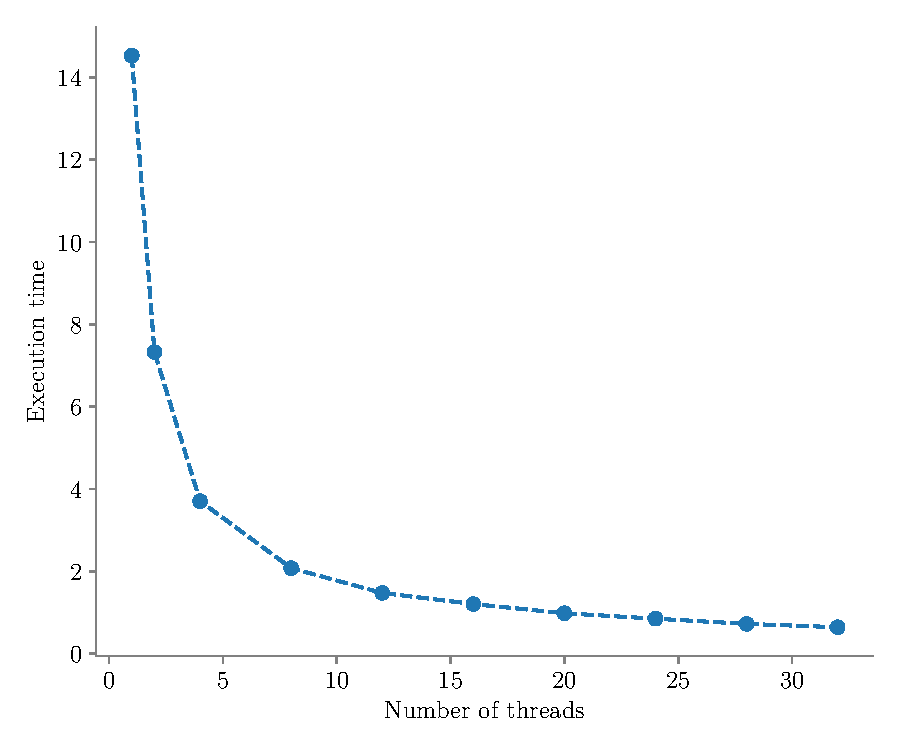
\includegraphics[width=0.8\textwidth]{dftw.pdf}
	\end{figure}
    
    \item \textit{Which performance optimizations would be suitable for DFT, other than parallelization with OpenMP? Explain, no need for implementing the optimizations.}
\end{enumerate}
\end{document}

